\documentclass[aspectratio=169]{beamer}

\mode<presentation> {
	\usetheme{Madrid}
	\setbeamertemplate{navigation symbols}{}
}

% ---------- 页尾 ----------
\setbeamertemplate{footline}{
	\begin{beamercolorbox}[wd=\paperwidth,ht=2.5ex,dp=1.25ex]{footline}
		\usebeamerfont{footline}\hspace{0.2cm}\insertshortinstitute%
		\hfill\insertshorttitle\hfill%
		\insertframenumber/\inserttotalframenumber\hspace{0.2cm}%
	\end{beamercolorbox}
}
\setbeamercolor{footline}{fg=orchiddark,bg=orchidlight!30}

% ---------- 二月兰紫配色 ----------
\definecolor{orchidpurple}{RGB}{146,39,143}
\definecolor{orchiddark}{RGB}{115,30,112}
\definecolor{orchidlight}{RGB}{230,210,230}
\definecolor{orchidteal}{RGB}{0,128,128}
\definecolor{orchidteallight}{RGB}{214,235,235}
\definecolor{orchidgold}{RGB}{198,140,0}
\definecolor{orchidgoldlight}{RGB}{250,240,216}

\setbeamercolor{structure}{fg=orchidpurple}
\setbeamercolor{palette primary}{fg=white,bg=orchidpurple}
\setbeamercolor{palette secondary}{fg=white,bg=orchiddark}
\setbeamercolor{palette tertiary}{fg=white,bg=orchidpurple}
\setbeamercolor{palette quaternary}{fg=white,bg=orchiddark}
\setbeamercolor{titlelike}{fg=white,bg=orchidpurple}
\setbeamercolor{frametitle}{fg=white,bg=orchidpurple}
\setbeamercolor{block title}{fg=white,bg=orchidpurple}
\setbeamercolor{block body}{fg=black,bg=orchidlight!22}
\setbeamercolor{item}{fg=orchidpurple}
\setbeamercolor{section in toc}{fg=orchiddark}
\setbeamercolor{block title alerted}{fg=white,bg=orchidteal}
\setbeamercolor{block body alerted}{fg=black,bg=orchidteallight}
\setbeamercolor{block title example}{fg=white,bg=orchidgold}
\setbeamercolor{block body example}{fg=black,bg=orchidgoldlight}
\setbeamercolor{think}{fg=orchiddark,bg=orchidlight!22}

% ---------- 章节过渡页 ----------
\AtBeginSection[]
{
	\begin{frame}
		\centering
		\vspace{1.5cm}
		{\usebeamerfont{title}\color{orchiddark}\insertsectionnumber.~\insertsectionhead}\\
		\vspace{0.5cm}
		{\color{orchidpurple}\rule{0.35\textwidth}{1.2pt}}
	\end{frame}
}

% ---------- 轻量想法/评注框 ----------
\setbeamercolor{think}{fg=orchiddark,bg=orchidlight!22}
\setbeamercolor{thinkg}{fg=orchiddark,bg=orchidgoldlight}
\newcommand{\remark}[2]{%
	\vspace{0.12cm}%
	\begin{beamercolorbox}[rounded=true,sep=6pt]{think}%
		{\color{orchidpurple}\textbf{#1}：}~#2%
	\end{beamercolorbox}%
}
\newcommand{\remarkg}[2]{%
	\vspace{0.12cm}%
	\begin{beamercolorbox}[rounded=true,sep=6pt]{thinkg}%
		{\color{orchidgold}\textbf{#1}：}~#2%
	\end{beamercolorbox}%
}
\newcommand{\remarkp}[2]{%
	\vspace{0.12cm}%
	{\color{orchidpurple}\textbf{#1}：}~#2\par%
}

\usepackage{graphicx}
\usepackage{booktabs}
\usepackage[UTF8,noindent]{ctexcap}
\usepackage[bookmarks=true]{hyperref}
\usepackage{amsmath,amssymb,bm}
\usepackage{tikz}
\usetikzlibrary{shapes.geometric,arrows,positioning}

% ---------- 快捷命令 ----------
\newcommand{\T}{^{\mathsf{T}}}
\newcommand{\R}{\mathbb{R}}
\newcommand{\mat}[1]{\bm{#1}}
\newcommand{\tbf}[1]{\textbf{#1}}

% ============================================================
%	以下为可修改区：标题 / 作者 / 单位 / 日期
% ============================================================

\title[063组分享]{《波浪能装置输出功率优化设计》赏析}
\author{魏舟}
\institute[南京理工大学]
{
	063组 \\
	\medskip
	\textit{wei\_zhou@njust.edu.cn}
}
\date{2026年8月}

% ============================================================
%	以下为正文示例，请按需替换
% ============================================================

\begin{document}

% ---------- 标题页 ----------
\begin{frame}
	\begin{center}
		\begin{beamercolorbox}[rounded=true,shadow=true,sep=8pt,center,wd=\textwidth]{title}
			\usebeamerfont{title}\inserttitle
		\end{beamercolorbox}
	\end{center}
	\vspace{0.5cm}
	\begin{columns}[c]
		\column{0.5\textwidth}
		\centering
		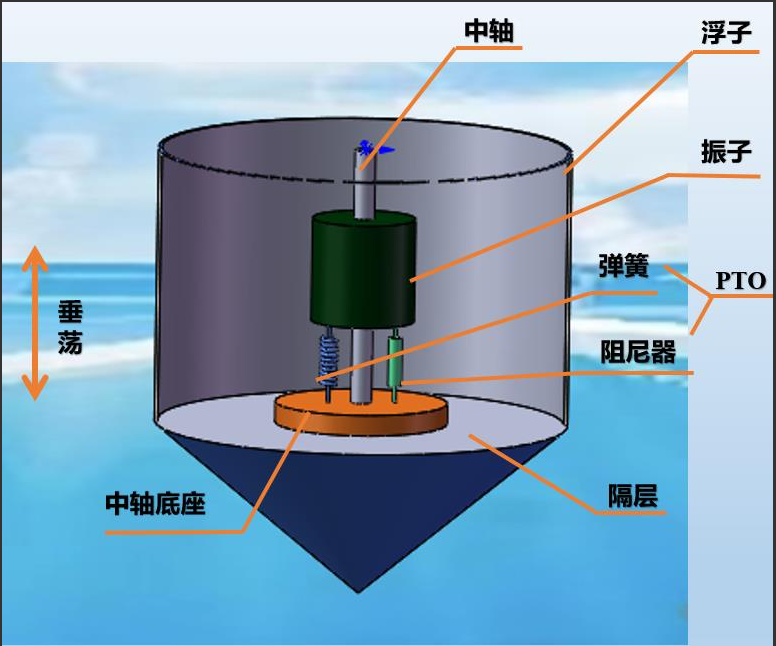
\includegraphics[width=0.9\textwidth]{Figure/波浪能装置示意图.png}

		\column{0.5\textwidth}
		\centering
		{\usebeamerfont{author}\usebeamercolor[fg]{author}\insertauthor}\\[0.4cm]
		{\usebeamerfont{institute}\usebeamercolor[fg]{institute}\insertinstitute}\\[0.4cm]
		{\usebeamerfont{date}\usebeamercolor[fg]{date}\insertdate}
	\end{columns}
\end{frame}

% ---------- 目录 ----------
\section*{目录}
\begin{frame}
	\frametitle{汇报提纲}
	\tableofcontents
\end{frame}
\setcounter{section}{0}


\section{文章结构}
\begin{frame}
	\frametitle{文章结构}
	\begin{center}
	\begin{tikzpicture}[
		box/.style={draw=orchidpurple, thick, rounded corners=3pt,
			minimum width=2.2cm, minimum height=1.2cm, align=center,
			fill=orchidlight!40},
		arrow/.style={-stealth, thick, orchidpurple}
	]
		\node[box] (a) at (0,0) {问题重述};
		\node[box] (b) at (4.8,0) {问题分析};
		\node[box] (c) at (9.6,0) {模型假设};
		\node[box] (d) at (9.6,-2.4) {模型的建立\\与求解};
		\node[box] (e) at (4.8,-2.4) {模型检验\\(分析)};
		\node[box, fill=orchidpurple, text=white] (f) at (0,-2.4) {总结};

		\draw[arrow] (a.east) -- (b.west);
		\draw[arrow] (b.east) -- (c.west);
		\draw[arrow] (c.south) -- (d.north);
		\draw[arrow] (d.west) -- (e.east);
		\draw[arrow] (e.west) -- (f.east);
	\end{tikzpicture}
	\end{center}
	这篇论文的骨架，就是我们课程里学的标准数模流程：从问题重述、建模求解，到检验、总结，一步没落。（有一个小问题，有些论文里面会在论文的开头画一个很好看的流程图，展示一下整体的建模思路，这篇文章没有，到底要不要来一个？）
\end{frame}

\section{标题分析}
\begin{frame}
	\frametitle{标题分析：一般AI撰写的标题}
	\small
	\begin{columns}[T]
		\column{0.58\textwidth}
		\setlength{\itemsep}{6pt}
		\begin{itemize}
			\item 《基于随机优化与动态规划的航空舱位分配与动态定价策略研究》
			\item 《基于嵌入式 MCU 的铝制工件表面缺陷检测系统》
			\item 《基于组合赋权-TOPSIS 与 Huff 引力模型的城市商圈消费活力评价与首店选址研究》
		\end{itemize}

		\column{0.42\textwidth}
		\begin{block}{一眼AI的原因}
			\begin{itemize}
				\item \textbf{模板化}：全是``基于……的研究''，一个模子刻的，看不出作者想解决啥。
				\item \textbf{术语堆砌}：动态规划、TOPSIS、Huff 模型，高级词一个接一个。
				\item \textbf{结构刻板}：永远是``方法 + 对象''。
				\item \textbf{用词空泛}：研究、优化、评价，大词多但指向弱，换个题也成立。
			\end{itemize}
		\end{block}
	\end{columns}

\end{frame}

\begin{frame}
	\frametitle{标题分析：本文的标题}
	\small
	\begin{columns}[T]
		\column{0.48\textwidth}
		\begin{block}{本文标题}
			\centering《波浪能装置输出功率优化设计》
		\end{block}
		\begin{alertblock}{结构拆解}
			\begin{itemize}
				\item \textbf{波浪能装置} --- 研究对象
				\item \textbf{输出功率} --- 优化目标
				\item \textbf{优化设计} --- 工作内容
			\end{itemize}
		\end{alertblock}

		\column{0.52\textwidth}
		\begin{exampleblock}{好在哪}
			\begin{itemize}
				\item 一句话就把``研究对象、优化目标、工作内容''说全了
				\item ``输出功率''直接点进标题，别人一看就知道你要干啥
				\item 不套``基于……''的模板，也没堆高级词
				\item 对象和任务都限定得死死的，不空
			\end{itemize}
		\end{exampleblock}
	\end{columns}
	\begin{center}
		这就是大道至简的感觉吗！
	\end{center}
\end{frame}

\section{摘要赏析}
\begin{frame}
	\frametitle{摘要赏析（一）：总述}
	\small
	\begin{block}{总述}
		本文在求波浪能最大输出功率设计中，通过受力分析，建立了浮子和振子的垂荡和纵摇运动模型，并通过四阶龙格库塔算法将建立的连续微分方程离散化处理，递推求出了相应时间内浮子和振子的垂荡纵摇运动情况。同时对功率的积分函数值以微小步长为底的梯形面积替代，通过遗传算法搜索参数，求出了最大输出功率和相应的最优阻尼系数，并对模型进行了检验和误差分析。
	\end{block}
	\medskip
	\remark{怎么写的}{这一段其实就是把全文讲了个大概：先说建了什么模型，再交代用了哪两个硬方法，然后给结果，最后补一句检验。顺序顺下来，评委应该能很快知道作者干了什么。我理解得比较粗，可能没说透。}
\end{frame}

\begin{frame}
	\frametitle{摘要赏析（二）：问题一、二}
	\scriptsize
	\begin{block}{问题一}
		首先，基于对坐标系灵活选取，通过牛顿第二定律，建立浮子和振子相互作用的垂荡运动模型。其次，根据模型及初始运动状态确定了垂荡运动的二元二阶力学微分方程。最后，利用改进的龙格库塔算法对处理后的方程进行迭代求解，得到了浮子和振子在前40个周期内时间间隔为0.2s的垂荡位移和速度。结果见表2。
	\end{block}
	\begin{block}{问题二}
		在浮子和振子相互作用的垂荡运动模型基础上，推导出了直线阻尼平均输出功率积分函数，建立了以垂荡运动装置的平均输出功率最大为目标的单目标优化模型。同时为求解该积分值，本文利用微小步长为底的梯形面积近似代替该函数值，且选取100s后的稳定状态作为区间求出平均输出功率，所需数值可由垂荡运动模型确定。最后，利用遗传算法搜索参数，确定在（1）条件下，最大平均输出功率为229.6819w，最优直线阻尼系数为37639；在（2）条件下，最大平均输出功率为230.0163w，最优直线阻尼系数为81478，幂指数为0.3377。
	\end{block}
	\medskip
	\remarkg{怎么写的}{\textbf{问题一}写得很``教学''：模型怎么建、方程长什么样、用什么算的、算出来啥，一步都不落。\textbf{问题二}顺着模型往优化上走，把功率写出来、定目标、用梯形面积把积分近似掉、再交给遗传算法去搜。我印象最深的是最后那串四位小数，个人觉得看着比较有说服力，当然也可能是我见识少。}
\end{frame}

\begin{frame}
	\frametitle{摘要赏析（三）：问题三、四}
	\scriptsize
	\begin{block}{问题三}
		首先，基于刚体转动的平行移轴定理和垂直轴定理、组合体重心计算公式，得到浮子和振子的纵摇运动的转动惯量函数。其次，基于牛顿第二定律，建立浮子和振子的纵摇运动模型。再进一步，确定了垂荡和纵摇之间的联系，得到该模型方程为四元二阶微分方程。最后，利用龙格库塔算法迭代求解该微分方程前40个波浪周期内时间间隔为0.2s的垂荡位移与速度、纵摇角位移与角速度。结果见表3。
	\end{block}
	\begin{block}{问题四}
		在浮子和振子的纵摇模型的基础上，同样推导出了旋转阻尼平均输出功率积分函数，在同时考虑垂荡和纵摇基础上，建立了以同时考虑垂荡和纵摇运动的平均输出功率最大为目标的单目标优化模型。为求解该积分函数，对连续功率函数进行与问题二相同的离散化处理，且选取100s后的稳定状态作为区间求出平均输出功率，所需数值可由垂荡、纵摇运动模型得出。最后，采用遗传搜索算法求解，确定最大平均输出功率为316.5807w，最优直线阻尼系数为58944，最优旋转阻尼系数为98227。
	\end{block}
	\medskip
	\remarkp{怎么写的}{\textbf{问题三、四}像是问题一、二的``加强版''：垂荡变垂荡加纵摇，直线阻尼变直线加旋转阻尼。方法还是龙格库塔和遗传算法，但模型从二维方程变成四元方程，难度确实上来了。我觉得这种复用自己方法的写法挺好的，评委读着也不累，不过也可能是我理解得浅。}
\end{frame}

\begin{frame}
	\frametitle{摘要赏析（四）：关键词}
	\begin{center}
		\vfill
		{\color{orchidpurple}\large\bfseries 振荡浮子式波浪能发电装置\ \ 垂荡\ \ 纵摇\ \ 四阶龙格库塔法\ \ 遗传搜索算法}
		\medskip
		\remark{怎么写的}{关键词挑了装置、运动形式、算法几个方面，覆盖面挺全。个人感觉这样挑检索起来挺方便，不知道是不是作者的用意，说得不对请大家指正。}
		\vfill
	\end{center}
\end{frame}

\begin{frame}
	\frametitle{总结}
	\scriptsize
	\begin{columns}[T]
		\column{0.5\textwidth}
		\begin{exampleblock}{要这样做}
			\begin{itemize}
				\item 第一段一句概括全文做了啥（建模、方法、结果、检验）
				\item 每个问题按"建模→求解→结果"顺序写
				\item 数字给具体值，不要"经计算得到最优解"
				\item 关键词从装置类型、运动形式、算法三方面挑
			\end{itemize}
		\end{exampleblock}
		\column{0.5\textwidth}
		\begin{alertblock}{不要这样做}
			\begin{itemize}
				\item 别抄题目的"背景意义"那段当摘要
				\item 别写"本文具有重要的理论意义和实际价值"这种空话
				\item 别把结果藏起来不写数字，评委翻半天找不到
				\item 别写"相关结果见表X、图X"，要给具体数
			\end{itemize}
		\end{alertblock}
	\end{columns}

\end{frame}

\section{问题重述思考}
\begin{frame}
	\frametitle{问题重述（一）：背景、结构与原理}
	\scriptsize
	\setlength{\parskip}{0pt}
	\remarkg{背景、结构与工作原理}{波浪能是新兴海洋清洁可再生能源，是国家能源发展战略的必然要求[1]。装置由浮子、振子、中轴、能量输出系统（PTO）组成。浮子由质量分布均匀的圆柱壳和圆锥壳组成，两壳体间隔层作中轴支撑面，PTO连接中轴底座与振子。波浪施加简谐激励力（矩），浮子带动振子摇荡，二者相对运动驱动阻尼器做功输出能量。}
	\begin{block}{题干条件 $\rightarrow$ 得到的信息}
		\setlength{\itemsep}{0pt}\setlength{\topsep}{0pt}\setlength{\partopsep}{0pt}
		\begin{columns}[T]
			\column{0.5\textwidth}
			\begin{itemize}
				\item 海水无粘无旋；线性周期微幅波 $\rightarrow$ 理想流体线性化，用线性波理论
				\item 四类水动力作用 $\rightarrow$ 牛顿第二定律受力项，列动力学方程
				\item 浮子质量均匀分布 $\rightarrow$ 质心、转动惯量可解析求
			\end{itemize}
			\column{0.5\textwidth}
			\begin{itemize}
				\item 振子穿中轴、圆柱体 $\rightarrow$ 约束为垂荡运动
				\item PTO弹簧+阻尼器，相对运动做功 $\rightarrow$ 目标：平均输出功率
				\item 忽略部件质量与摩擦 $\rightarrow$ 仅对浮子、振子建模
			\end{itemize}
		\end{columns}
	\end{block}
	\remarkp{赏析}{开头交代了为什么要做这件事，还引了文献；中间把装置部件一个个说清楚；原理那句把``波浪推浮子、浮子带动振子、阻尼做功发电''讲明白了。建模要用的信息其实都藏在这几段里，我个人是这样理解的，可能不全面。}
\end{frame}

\begin{frame}
	\frametitle{教程：论文开头三句话怎么分配}
	\scriptsize
	\begin{block}{逐句拆开看}
		\begin{itemize}
			\item \textbf{第1句（意义）}：``波浪能是新兴海洋清洁可再生能源，是国家能源发展战略的必然要求[1]。''——先交代\textbf{你研究这事为啥重要}，一句话就够了，别写成长篇综述
			\item \textbf{第2句（装置）}：``装置由浮子、振子、中轴、能量输出系统（PTO）组成……''——交代\textbf{你研究的对象长什么样}，像报菜名一样把部件说全，后文要用的名词这里第一次出现
			\item \textbf{第3句（原理）}：``波浪施加简谐激励力（矩），浮子带动振子摇荡，二者相对运动驱动阻尼器做功输出能量。''——交代\textbf{这东西怎么工作}，用''原因→过程→结果''一条链串起来
		\end{itemize}
	\end{block}

\end{frame}

\begin{frame}
	\frametitle{问题重述（二）：问题一、问题二}
	\scriptsize
	\begin{block}{问题一}
		已知直线阻尼器的阻尼力同浮子和振子的相对速度成正比；波浪激励力满足 $f\cos\omega t$。建立浮子与振子的垂荡运动模型，并据此分别计算直线阻尼器阻尼系数为常数和随浮子与振子相对速度变化两种情形下，浮子和振子在规定时刻的垂荡位移和速度。
	\end{block}
	\begin{block}{问题二}
		仅考虑垂荡运动，以PTO系统平均输出功率最大为目标，建立直线阻尼器最优阻尼系数的数学模型，并根据所给参数求出以下两种约束条件下装置的最大输出功率及相应的最优阻尼系数：（1）阻尼系数为常量，取值范围为 $[0,100000]$；（2）阻尼系数为变量，与浮子和振子相对速度的绝对值的幂成正比，比例系数取值范围为 $[0,100000]$，幂指数取值范围为 $[0.1,1]$。
	\end{block}
	\medskip
	\remark{赏析}{问题一先让建模型、算位移算速度，算是热身；问题二才求功率最大的阻尼系数，还分常系数和变系数两种情况，参数范围都给好了。我读的时候觉得他们把约束写得清清楚楚，我们照着做就行，就像在解振动理论的期末考试试题一样，这点做得挺清楚。}
\end{frame}

\begin{frame}
	\frametitle{问题重述（三）：问题三、问题四}
	\scriptsize
	\begin{block}{问题三}
		同时考虑垂荡和纵摇运动，振子既随中轴转动，又沿中轴滑动，直线阻尼器、旋转阻尼器均存在能量输出。给定波浪激励力和激励力矩 $f\cos\omega t,\ L\cos\omega t$，建立浮子与振子的垂荡和纵摇运动模型，按给定参数设定初始条件，计算前40个波浪周期内时间间隔为0.2s的垂荡位移与速度、纵摇角位移与角速度。
	\end{block}
	\begin{block}{问题四}
		同时考虑垂荡和纵摇运动，以PTO系统最大输出功率为目标，建立直线阻尼器、旋转阻尼器最优阻尼系数的数学模型，并求出当二者阻尼系数取值范围均为 $[0,100000]$、波浪频率为 $1.9806\,\mathrm{s}^{-1}$ 时，装置的最大输出功率及相应的最优阻尼系数。
	\end{block}
	\medskip
	\remarkg{赏析}{问题三难度明显上来了：又垂荡又纵摇，振子一边转一边滑，还冒出个旋转阻尼；计算要求也细到前40个周期、0.2秒一个点。问题四再把两个阻尼系数一起优化、给定频率。说实话我看到这儿有点压力，感觉让我们自己做，会有点困难。}
\end{frame}

\begin{frame}
	\frametitle{问题重述（四）：总结}
	\scriptsize
	\begin{block}{重述的写作结构}
		\begin{itemize}
			\item 背景（意义+文献[1]）$\rightarrow$ 结构（部件清单）$\rightarrow$ 原理（能量输出链条）$\rightarrow$ 四个递进问题
			\item 前三段为后文建模``备料''：质量分布、简谐激励、阻尼做功全部埋在其中
		\end{itemize}
	\end{block}
	\begin{block}{四个问题：两轮递进}
		\begin{center}
		\begin{tikzpicture}[
			qbox/.style={draw=orchidpurple, thick, rounded corners=3pt,
				minimum width=2.5cm, minimum height=0.9cm, align=center,
				fill=orchidlight!35, font=\scriptsize},
			arrow/.style={-stealth, thick, orchidpurple},
			lab/.style={font=\scriptsize\bfseries, orchidpurple}
		]
			\node[qbox] (q1) at (0,0) {问题一\\建垂荡模型求运动};
			\node[qbox] (q2) at (5.6,0) {问题二\\垂荡优化求功率};
			\node[qbox] (q3) at (0,-2.4) {问题三\\建双运动模型求运动};
			\node[qbox] (q4) at (5.6,-2.4) {问题四\\双运动优化求功率};
			\draw[arrow] (q1.east) -- (q2.west);
			\draw[arrow] (q3.east) -- (q4.west);
			\draw[arrow] (q1.south) -- (q3.north);
			\draw[arrow] (q2.south) -- (q4.north);
			\node[lab, anchor=east] at (-1.7,0) {第一轮：仅垂荡};
			\node[lab, anchor=east] at (-1.7,-2.4) {第二轮：垂荡+纵摇};
		\end{tikzpicture}
		\end{center}
	\end{block}
	\remarkp{赏析}{先简单后复杂一层层加码，不过也可能我想多了。}
\end{frame}

\begin{frame}
	\frametitle{总结：问题重述别抄题目}
	\scriptsize
	\begin{columns}[T]
		\column{0.5\textwidth}
		\begin{exampleblock}{要这样做}
			\begin{itemize}
				\item 背景、结构、原理分三段，各司其职
				\item 四问用一句概括，让读者先有全局
				\item 把参数、范围写具体，不要"在给定条件下"
				\item 四问之间有递进关系就说清楚
			\end{itemize}
		\end{exampleblock}
		\column{0.5\textwidth}
		\begin{alertblock}{不要这样做}
			\begin{itemize}
				\item 原样粘贴题目原文，一字不改
				\item 把题目的"海洋能源背景"抄两页
				\item 问题之间孤立写，看不出谁是谁的铺垫
				\item 参数用"详见附件"带过，回头找很累
			\end{itemize}
		\end{alertblock}
	\end{columns}

\end{frame}

\section{问题分析思考}
\begin{frame}
	\frametitle{问题分析（一）：问题一分析}
	\scriptsize
	\begin{block}{原文}
		问题一需要根据波浪激励力建立浮子与振子运动模型。本题难点在于准确反映浮子和振子振动的物理过程。对此，灵活选取坐标系，基于牛顿第二定律，建立浮子和振子相对运动的二阶二元微分方程。继而对微分方程采用改进的四阶龙格库塔算法求解，实现了高精度的要求。
	\end{block}
	\medskip
	\remark{赏析}{作者先说难点在``怎么把物理过程反映准''，再给办法：选坐标系、牛顿定律、龙格库塔。我觉得能做到``点出难点、给出对策''就不错了，我们写的时候经常是难点说不清楚。}
\end{frame}

\begin{frame}
	\frametitle{问题分析（二）：问题二分析}
	\scriptsize
	\begin{block}{原文}
		在问题一的基础上，需要利用附件三和附件四的参数值，求出指定情况下能使系统平均输出功率最大的最优阻尼系数。本题通过选定合理的时间区间，推导平均功率函数，继而建立直线阻尼器阻尼系数的优化模型，利用龙格库塔法粗略寻优后采用遗传算法，分别求出阻尼系数为常量、阻尼系数随相对速度变化时两种情况下的最大平均输出功率以及对应的最优阻尼系数。
	\end{block}
	\medskip
	\remarkg{赏析}{这一问接着上一问，把功率算出来再优化阻尼。作者先选定一段稳定时间算平均功率，再建优化模型，龙格库塔粗找一遍、遗传算法精修。这个``先粗后精''的思路我挺受启发，坦白说让我自己想，未必想得到。}
\end{frame}

\begin{frame}
	\frametitle{问题分析（三）：问题三分析}
	\scriptsize
	\begin{block}{原文}
		本题需进一步考虑纵摇运动。对此基于牛顿第二定律，建立纵摇运动模型，并利用组合体的重心计算公式、刚体转动的垂直轴定理和平行移轴定理，实现振荡浮子式波浪能发电装置的转动惯量的计算。最后用改进的四阶龙格库塔算法实现问题三的求解。
	\end{block}
	\medskip
	\remarkp{赏析}{问题三加了纵摇，多出来的活是算转动惯量——重心公式、垂直轴定理、平行移轴定理都用上了。我看到这儿才发现这题还要用理论力学，坦白讲，让我自己做的话可能就卡在这一步了。}
\end{frame}

\begin{frame}
	\frametitle{问题分析（四）：问题四分析}
	\scriptsize
	\begin{block}{原文}
		在问题三的基础上，针对直线阻尼器和旋转阻尼器的系数均为常量的情况，需要确定指定取值范围内，使平均输出功率最大的最优阻尼系数。对此，建立阻尼系数的优化模型，选取系统稳定响应后的一段时间计算垂荡运动、纵摇运动的平均输出功率，利用龙格库塔法粗略寻优后，采用遗传算法快速求解得到最大输出功率和相应的最优阻尼系数。
	\end{block}
	\medskip
	\remark{赏析}{这个细节我以前没注意过。}
\end{frame}

\begin{frame}
	\frametitle{问题分析（五）：总结}
	\scriptsize
	\setlength{\parskip}{0pt}
	\begin{itemize}
		\item 每题都是``承上（在上一问基础上）+ 建模 + 求解工具''三步展开
		\item 建模/优化交替：问题一、三\textbf{建运动模型求运动}，问题二、四\textbf{建优化模型求功率}
	\end{itemize}
	\vspace{0.15cm}
	\begin{center}
	\begin{tikzpicture}[
		mbox/.style={draw=orchidpurple, thick, rounded corners=3pt,
			minimum width=3.0cm, minimum height=0.95cm, align=center,
			fill=orchidlight!35, font=\scriptsize},
		arrow/.style={-stealth, thick, orchidpurple},
		tlab/.style={font=\scriptsize\bfseries, orchidpurple}
	]
		\node[mbox] (a1) at (0,0) {受力分析\\牛顿第二定律};
		\node[mbox] (b1) at (4.1,0) {运动方程};
		\node[mbox] (c1) at (8.2,0) {四阶龙格库塔\\求运动};
		\node[mbox] (a2) at (0,-2.2) {目标 + 约束};
		\node[mbox] (b2) at (4.1,-2.2) {优化模型};
		\node[mbox] (c2) at (8.2,-2.2) {遗传算法\\求最优};
		\draw[arrow] (a1.east) -- (b1.west);
		\draw[arrow] (b1.east) -- (c1.west);
		\draw[arrow] (a2.east) -- (b2.west);
		\draw[arrow] (b2.east) -- (c2.west);
		\node[tlab] at (-0.2,1.0) {建运动模型：问题一、三};
		\node[tlab] at (-0.2,-3.2) {建优化模型：问题二、四};
	\end{tikzpicture}
	\end{center}
	\remarkg{赏析}{方法就那几样，来回用，但是细节的地方又有区别，这大概是这篇最厉害的地方。理解得浅，说错的地方请大家指正。}
\end{frame}

\begin{frame}
	\frametitle{教程：问题分析别写成"习题解答"}
	\scriptsize
	\begin{columns}[T]
		\column{0.5\textwidth}
		\begin{exampleblock}{要这样做}
			\begin{itemize}
				\item 每问都交代"站在哪一基础上"
				\item 先点难点，再给对策，别一上来就丢公式
				\item 把方法工具箱亮出来（牛顿定律、龙格库塔、遗传算法）
				\item 几问之间说清楚怎么递进
			\end{itemize}
		\end{exampleblock}
		\column{0.5\textwidth}
		\begin{alertblock}{不要这样做}
			\begin{itemize}
				\item 把问题陈述复读一遍当分析
				\item 每问孤立写，看不出前后关系
				\item "本题采用改进的龙格库塔算法求解"——为什么改进、什么精度，不说
				\item 用了什么方法不跟后面的求解连上
			\end{itemize}
		\end{alertblock}
	\end{columns}
	\remark{跟你们说}{问题分析是你告诉评委"你想怎么解"的地方。这篇最好的一点是每问都交代了"难点在哪、怎么破"，给后面建模铺路。}
\end{frame}

\section{模型假设和符号表思考}
\begin{frame}
	\frametitle{模型假设和符号表（一）：模型假设}
	\scriptsize
	\setlength{\parskip}{0pt}
	\begin{itemize}
		\item 波浪为线性周期微幅波，忽略波面升高 $\rightarrow$ 波浪力线性化，可用线性波理论
		\item 海水为理想流体，无粘、无旋、不可压缩 $\rightarrow$ 可用势流理论描述
		\item 忽略纵摇运动对垂荡运动的影响 $\rightarrow$ 问题一、二可先只考虑垂荡（解耦）
		\item 忽略中轴、底座、隔层及PTO的质量和各种摩擦 $\rightarrow$ 只对浮子、振子两刚体建模
	\end{itemize}
	\medskip
	\remarkp{赏析}{写假设最要紧的是每一条都要在模型里``对得上号''——省了哪一项、为什么能省，作者处理得清楚，值得学。}
\end{frame}

\begin{frame}
	\frametitle{模型假设和符号表（二）：符号表赏析}
	\scriptsize
	\remark{符号表的格式}{这篇文章里符号表格式很规整：共\textbf{三栏}，第一栏\textbf{符号}、第二栏\textbf{意义}、第三栏\textbf{单位}，表头和正文全部\textbf{居中}排列。符号用斜体字母，含义用文字说明，单位用正体，三栏齐备，读者不用回正文翻找含义。}
	\begin{center}
		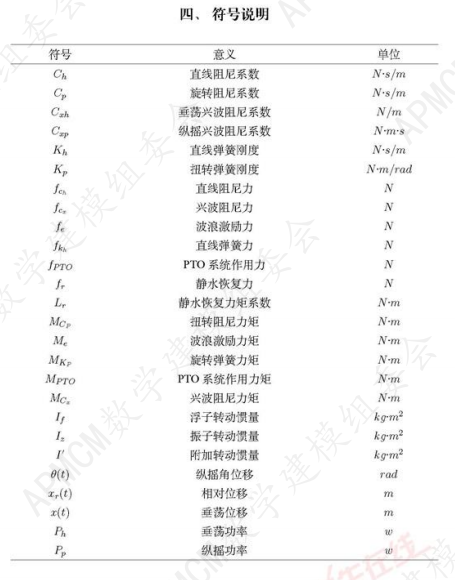
\includegraphics[width=0.65\textwidth]{Figure/符号表.png}\\
		\small 图：本文符号表
	\end{center}
\end{frame}




\section{模型的建立与求解思考}
\begin{frame}
	\frametitle{建模思路总览：这篇的建模就六步}
	\scriptsize
	\begin{center}
	\begin{tikzpicture}[
		stepbox/.style={draw=orchidpurple, thick, rounded corners=3pt,
			minimum width=1.75cm, minimum height=1.5cm, align=center,
			fill=orchidlight!35, font=\scriptsize},
		arrow/.style={-stealth, thick, orchidpurple}
	]
		\node[stepbox] (a) at (0,0) {1 审题\\把题干翻成\\建模需求};
		\node[stepbox] (b) at (2.35,0) {2 物理建模\\受力分析\\列方程};
		\node[stepbox] (c) at (4.7,0) {3 数值求解\\转一阶\\龙格库塔};
		\node[stepbox] (d) at (7.05,0) {4 目标约束\\平均功率\\阻尼范围};
		\node[stepbox] (e) at (9.4,0) {5 寻优\\粗扫+遗传算法};
		\node[stepbox] (f) at (11.75,0) {6 检验\\周期+扰动};
		\draw[arrow] (a.east) -- (b.west);
		\draw[arrow] (b.east) -- (c.west);
		\draw[arrow] (c.east) -- (d.west);
		\draw[arrow] (d.east) -- (e.west);
		\draw[arrow] (e.east) -- (f.west);
	\end{tikzpicture}
	\end{center}
	四问不是四个独立的题，而是这六步在\textbf{建模/优化} $\times$ \textbf{单运动/双运动}里的循环。下面逐页展开。
\end{frame}

\begin{frame}
	\frametitle{问题一·建模（1/6）：坐标系与受力分析}
	\scriptsize
	\begin{columns}[T]
		\column{0.6\textwidth}
		\begin{block}{坐标系的选取}
			\begin{itemize}
				\item 本题只考虑竖直\textbf{垂荡}（$Z$ 轴）与绕 $Y$ 轴\textbf{纵摇}两个自由度
				\item \textbf{大地系} $OXYZ$：原点取静止时浮子重心，固定不动
				\item \textbf{固体系} $oxyz$：原点取静止时振子中心对应的浮子上一点，随浮子运动
				\item 振子相对位移 $x_r(t)=x_2(t)-x_1(t)$
			\end{itemize}
		\end{block}
		\begin{block}{受力分析（仅垂荡）}
			\begin{itemize}
				\item \textbf{浮子}：波浪激励力 $f\cos\omega t$、附加惯性力、兴波阻尼力、静水恢复力 $-\rho g A x_1$、PTO 作用力
				\item \textbf{振子}：PTO 作用力（弹簧力 $f_k$ + 阻尼力 $f_d$）
			\end{itemize}
		\end{block}
		\column{0.4\textwidth}
		\begin{center}
			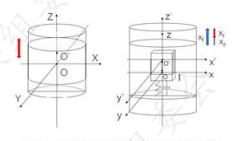
\includegraphics[width=\textwidth]{Figure/大地坐标系和固体坐标系示意图.png}\\
			\scriptsize 大地坐标系与固体坐标系（示意）
		\end{center}
	\end{columns}
\end{frame}

\begin{frame}
	\frametitle{问题一·建模（2/6）：垂荡运动方程}
	\scriptsize
	\begin{columns}[T]
		\column{0.6\textwidth}
		\begin{block}{PTO 系统作用力}
			\begin{itemize}
				\item 直线弹簧力：$f_k=-K\big(x_1(t)-x_2(t)\big)$，与相对位移成正比，$K$ 为弹簧刚度
				\item 直线阻尼力：$f_d=-C\big(\dot x_1(t)-\dot x_2(t)\big)$，与相对速度成正比，$C$ 为阻尼系数
			\end{itemize}
		\end{block}
		\begin{block}{牛顿第二定律列方程}
			浮子：$(m_1+m_a)\ddot x_1(t) = f\cos\omega t + f_d + f_k - \rho g A x_1$\\
			振子：$m_2\ddot x_2(t) = -f_d - f_k$\\
			代入 $f_k,f_d$ 整理后得到关于 $x_1,x_2$ 的\textbf{二元二阶常微分方程组}
		\end{block}
		\column{0.4\textwidth}
		\begin{center}
			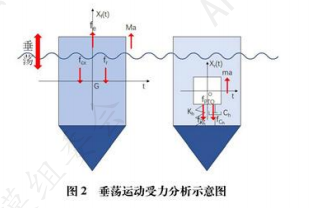
\includegraphics[width=\textwidth]{Figure/垂荡运动受力分析示意图.png}\\
			\scriptsize 浮子与振子受力分析（示意）
		\end{center}
	\end{columns}
	\remarkp{我的想法}{列方程时我犯过错：忘了振子上的力是浮子的反力，方向写反结果全错。想明白``作用力与反作用力''后就通了。}
\end{frame}

\begin{frame}
	\frametitle{问题一·建模（3/6）：四阶龙格库塔求解}
	\scriptsize
	\begin{columns}[T]
		\column{0.5\textwidth}
		\begin{block}{为什么自己改进}
			\begin{itemize}
				\item 要求前 40 周期、0.2s 间隔的位移和速度，MATLAB 自带 ode45 不便精确控制采样
				\item 直接对\textbf{四阶龙格库塔}（截断误差 $O(h^5)$）改进，精度与采样同时满足
			\end{itemize}
		\end{block}
		\begin{block}{二阶转一阶}
			令 $u_1=x_1,\ u_2=\dot x_1,\ v_1=x_2,\ v_2=\dot x_2$，把二元二阶方程组改写为\textbf{一阶四元方程组}
		\end{block}
		\begin{block}{递推公式}
			$y_{n+1}=y_n+\frac{h}{6}(k_1+2k_2+2k_3+k_4)$\\
			$k_1=f(t_n,y_n)$，$k_2=f(t_n+\frac{h}{2},y_n+\frac{h}{2}k_1)$\\
			$k_3=f(t_n+\frac{h}{2},y_n+\frac{h}{2}k_2)$，$k_4=f(t_n+h,y_n+hk_3)$
		\end{block}
		\column{0.5\textwidth}
		\begin{block}{参数与初值}
			\begin{itemize}
				\item 步长 $h=10^{-4}$，递推长度 40 个波浪周期
				\item 初值（静水平衡）：$x_1(0)=x_2(0)=0$，$\dot x_1(0)=\dot x_2(0)=0$
				\item 按 0.2s 间隔采样，保存结果
			\end{itemize}
		\end{block}

	\end{columns}
\end{frame}


\begin{frame}
	\frametitle{问题二·建模（1/6）：平均功率函数}
	\scriptsize
	\begin{block}{瞬时功率}
		平动功率 $P=F\cdot v$，PTO 直线阻尼器消耗的瞬时功率为
		\begin{center}
			$P(t)=C\big(\dot x_1(t)-\dot x_2(t)\big)^2$
		\end{center}
	\end{block}
	\begin{block}{平均功率}
		取系统振动\textbf{稳态响应后}的一段时间 $[t_1,t_2]$ 求平均：
		\begin{center}
			$P_{avg}=\dfrac{1}{t_2-t_1}\int_{t_1}^{t_2} C\,(\dot x_1-\dot x_2)^2\,dt$
		\end{center}
		$C\in[0,100000]$；题 1.(1) 中 $C$ 为常量，题 1.(2) 中 $C=\alpha\,|v_r|^{\beta}$
	\end{block}
	\remarkg{我的想法}{平均功率的定义看着简单，但有个细节我一开始没注意：为什么只取稳态段求平均？因为前面有一段瞬态，功率不稳定，取平均会把结果带偏。我自己画出功率曲线才真正理解这个取舍。}
\end{frame}

\begin{frame}
	\frametitle{问题二·建模（2/6）：优化模型建立}
	\scriptsize
	\begin{block}{目标函数}
		$\max\limits_{C}\ P_{avg}(C)$，其中 $P_{avg}=\dfrac{1}{t_2-t_1}\displaystyle\int_{t_1}^{t_2} C\big(\dot x_1-\dot x_2\big)^2\,dt$
	\end{block}
	\begin{block}{约束条件}
		\begin{itemize}
			\item \textbf{运动方程约束}：垂荡运动模型（问题一的方程组）
			\item \textbf{情况 (1)}：$C$ 为常量，$C\in[0,100000]$
			\item \textbf{情况 (2)}：$C=\alpha\,|v_r|^{\beta}$，$\alpha\in[0,100000]$，$\beta\in[0.1,1]$
			\item 波浪激励 $f\cos\omega t$，初值取静水平衡
		\end{itemize}
	\end{block}
	\remarkp{我的想法}{约束范围论文都给了，照着就能算，省得自己猜。我之前写优化题，约束老是含糊，评委看着就摇头。}
\end{frame}

\begin{frame}
	\frametitle{问题二·建模（3/6）：数值求解——梯形法}
	\scriptsize
	\begin{columns}[T]
		\column{0.5\textwidth}
		\begin{block}{功率积分离散化}
			\begin{itemize}
				\item 用\textbf{梯形法}求积分：步长足够小时，把连续函数用梯形面积之和近似
				\item 时间步长取 $10^{-4}$，满足精度要求
				\item 因前期位移不稳定，截取稳态段 $[100,180]$s 求平均功率
			\end{itemize}
		\end{block}
		\begin{block}{先粗后精的寻优}
			\begin{itemize}
				\item \textbf{粗略寻优}：增大阻尼系数遍历步长，得到功率随阻尼系数的分布
				\item \textbf{遗传算法精求}：避免局部最优、并行搜索、按概率选最优，迭代 200 次
			\end{itemize}
		\end{block}
		\column{0.5\textwidth}
		\begin{center}
			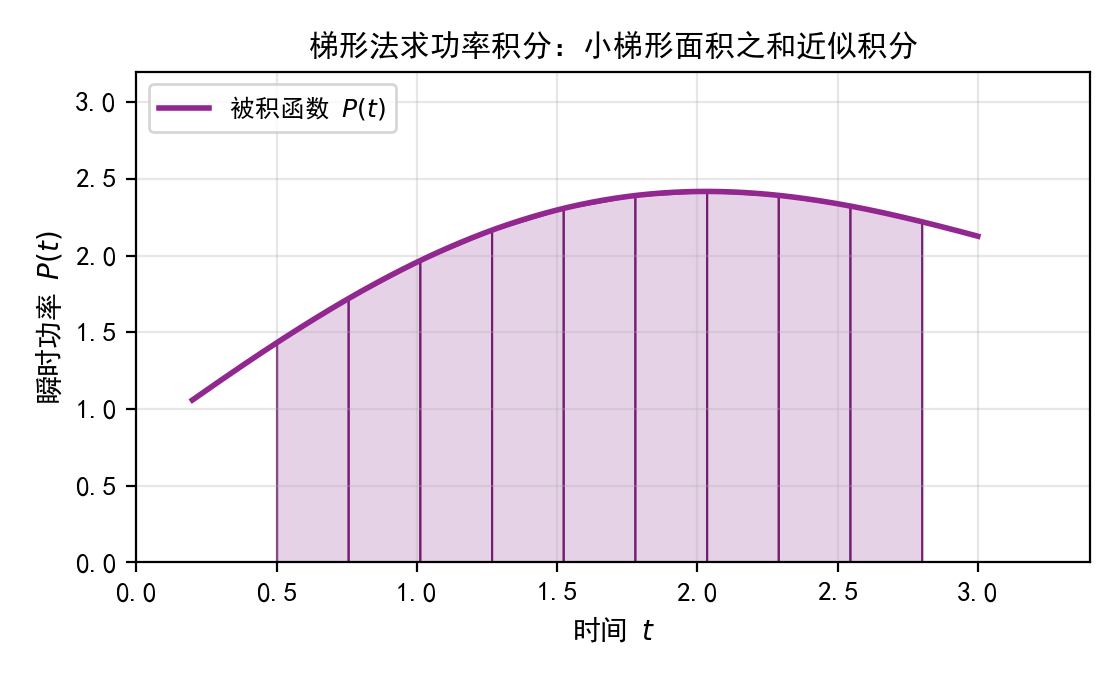
\includegraphics[height=0.3\textheight]{Figure/fig_sim_04.png}
		\end{center}
		\remark{我的想法}{梯形法是我这次重点学的对象：积分不会算没关系，用一堆小梯形去近似，步长越小越接近真值。更妙的是``先粗扫、再遗传算法精找''的组合，直接暴力遍历太慢，遗传算法又能跳出局部最优。这个思路我记下了，以后做优化题都能用。}
	\end{columns}
\end{frame}


\begin{frame}
	\frametitle{问题三·建模（1/4）：转动惯量计算}
	\scriptsize
	\begin{columns}[T]
		\column{0.56\textwidth}
		\begin{block}{先定转轴、再求重心}
			\begin{itemize}
				\item 纵摇时物体绕 $y$ 轴近似\textbf{穿过重心}，因此先确定浮子重心位置
				\item 浮子外壳看作\textbf{圆面 + 圆柱侧面 + 圆锥侧面}的组合体，重心用组合体重心公式 $\bar z=\dfrac{\sum m_i z_i}{\sum m_i}$
			\end{itemize}
		\end{block}
		\begin{block}{平行移轴与垂直轴定理}
			\begin{itemize}
				\item \textbf{平行移轴定理}：$I=I_C+md^2$（$d$ 为平行轴到质心轴距离）
				\item \textbf{垂直轴定理}：薄片对垂直轴惯量 $=$ 平面内两正交轴惯量之和
				\item 得浮子 $I_1=58289.43\,\mathrm{kg\cdot m^2}$；振子惯量随相对位移变化 $I_2=202.75+243.3\,(0.8+x_r(t))^2$
			\end{itemize}
		\end{block}
		\column{0.44\textwidth}
		\begin{center}
			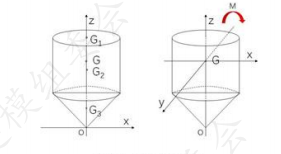
\includegraphics[height=0.26\textheight]{Figure/重心位置的确定.png}\\
			\scriptsize 组合体重心位置（示意）\\[2pt]
			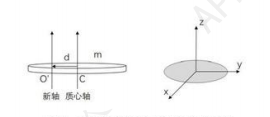
\includegraphics[height=0.19\textheight]{Figure/平行移轴和垂直轴定理.png}\\
			\scriptsize 平行移轴与垂直轴定理（示意）
		\end{center}
	\end{columns}
\end{frame}

\begin{frame}
	\frametitle{问题三·建模（2/4）：纵摇运动方程}
	\scriptsize
	\begin{columns}[T]
		\column{0.6\textwidth}
		\begin{block}{受力分析与 PTO 力矩}
			\begin{itemize}
				\item \textbf{浮子}受：波浪激励力矩 $L\cos\omega t$、附加惯性力矩、兴波阻尼力矩、静水恢复力矩 $M_s=-L_s\theta_1$、PTO 作用力矩；\textbf{振子}只受 PTO 作用力矩
				\item 旋转弹簧力矩：$M_k=-K_t\big(\theta_1(t)-\theta_2(t)\big)$
				\item 扭转阻尼力矩：$M_d=-C_t\big(\dot\theta_1(t)-\dot\theta_2(t)\big)$
			\end{itemize}
		\end{block}
		\begin{block}{牛顿第二定律（转动）}
			浮子：$(I_1+I_a)\ddot\theta_1 = L\cos\omega t + M_k + M_d - L_s\theta_1$\\
			振子：$I_2\ddot\theta_2 = -M_k - M_d$\\
			与问题一垂荡方程\textbf{联立} $\Rightarrow$ \textbf{四元二阶微分方程组}
		\end{block}
		\column{0.4\textwidth}
		\begin{center}
			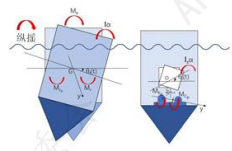
\includegraphics[width=\textwidth]{Figure/纵摇运动受力分析示意图.png}\\
			\scriptsize 纵摇受力分析（示意）
		\end{center}
	\end{columns}
	\remarkg{我的想法}{多自由度的题如果解耦了，其实就是单自由度复制几份再串起来，会一个就差不多会一串了。}
\end{frame}

\begin{frame}
	\frametitle{问题三·建模（3/4）：求解}
	\scriptsize
	\begin{block}{转一阶多元方程组}
		\begin{itemize}
			\item 把垂荡 + 纵摇的四元二阶方程组改写为\textbf{一阶八元方程组}
			\item 初值（静水平衡）：各（角）位移、速度、角速度均为 0
		\end{itemize}
	\end{block}
	\begin{block}{龙格库塔递推}
		\begin{itemize}
			\item 与问题一同法，用\textbf{四阶龙格库塔}递推（步长 $10^{-4}$）
			\item 递推前 40 个波浪周期，按 0.2s 间隔采样
			\item 输出浮子、振子的\textbf{位移、速度、角位移、角速度}四组量
		\end{itemize}
	\end{block}
	\remarkp{我的想法}{方法用熟一套，四问都能啃下来，比啥都现学强。}
\end{frame}

\begin{frame}
	\frametitle{问题三·结果：前 40 周期垂荡与纵摇运动}
	\scriptsize
	\begin{columns}[c]
		\column{0.5\textwidth}
		\begin{center}
			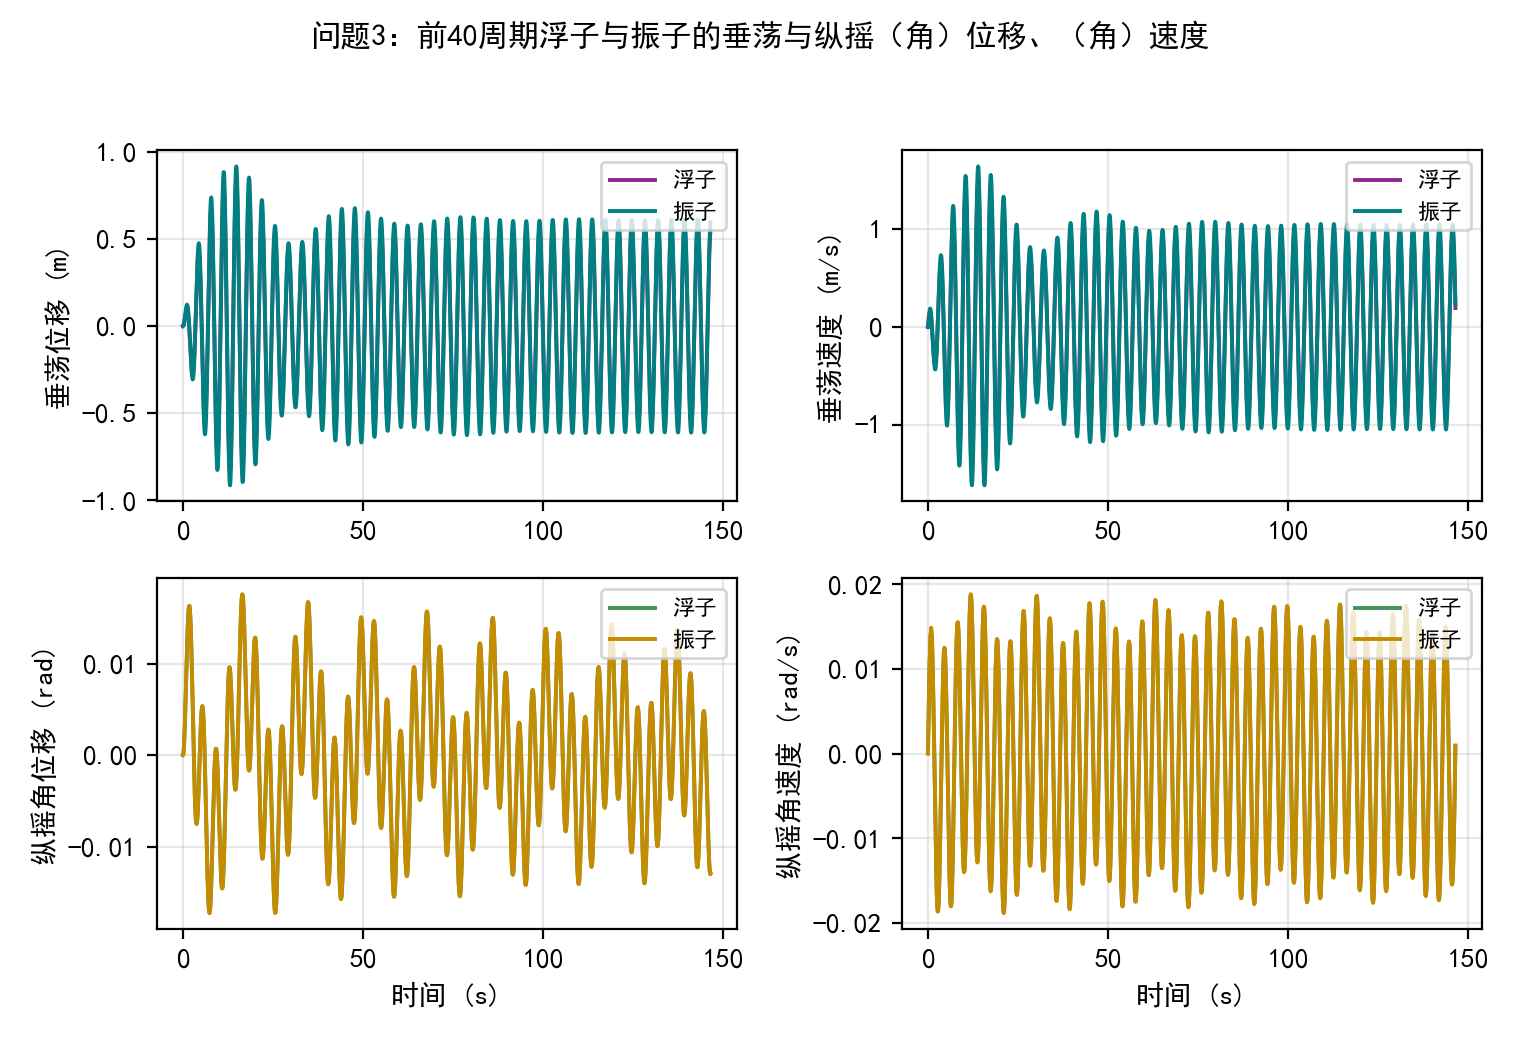
\includegraphics[width=\textwidth]{Figure/fig_sim_07.png}
		\end{center}
		\column{0.5\textwidth}
		\remark{我的想法}{最让我意外的是纵摇角只有 0.018 rad，特别小。这正好解释问题四``旋转阻尼几乎不影响功率''——纵摇动得少，旋转阻尼使不上劲。}
	\end{columns}
\end{frame}

\begin{frame}
	\frametitle{问题四·建模（1/3）：功率函数推导}
	\scriptsize
	\begin{block}{瞬时功率}
		转动功率 $P=M\cdot\omega$；PTO 总瞬时功率 = 直线阻尼功率 + 旋转阻尼功率
		\begin{center}
			$P(t)=C\big(\dot x_1-\dot x_2\big)^2 + C_t\big(\dot\theta_1-\dot\theta_2\big)^2$
		\end{center}
	\end{block}
	\begin{block}{平均功率}
		取稳态响应后的一段时间 $[t_1,t_2]$ 求平均：
		\begin{center}
			$P_{avg}=\dfrac{1}{t_2-t_1}\displaystyle\int_{t_1}^{t_2}\Big[C\big(\dot x_1-\dot x_2\big)^2 + C_t\big(\dot\theta_1-\dot\theta_2\big)^2\Big]dt$
		\end{center}
	\end{block}
\end{frame}

\begin{frame}
	\frametitle{问题四·建模（2/3）：优化模型建立}
	\scriptsize
	\begin{block}{目标函数}
		\begin{center}
			$\max\limits_{C,\,C_t}\ P_{avg}(C,C_t)$
		\end{center}
	\end{block}
	\begin{block}{约束条件}
		\begin{itemize}
			\item \textbf{运动方程约束}：垂荡 + 纵摇联立的四元二阶方程组
			\item 直线阻尼系数 $C\in[0,100000]$，旋转阻尼系数 $C_t\in[0,100000]$
			\item 波浪频率 $\omega=1.9806\,\mathrm{s^{-1}}$；初值取静水平衡
		\end{itemize}
	\end{block}
	\remarkp{我的想法}{决策量从问题二的一个变成两个（$C$ 和 $C_t$），求解框架完全相同。看懂问题二，问题四就懂了一半。}
\end{frame}

\begin{frame}
	\frametitle{问题四·结果：双阻尼系数下的功率分布（三维）}
	\scriptsize
	\begin{columns}[c]
		\column{0.5\textwidth}
		\begin{center}
			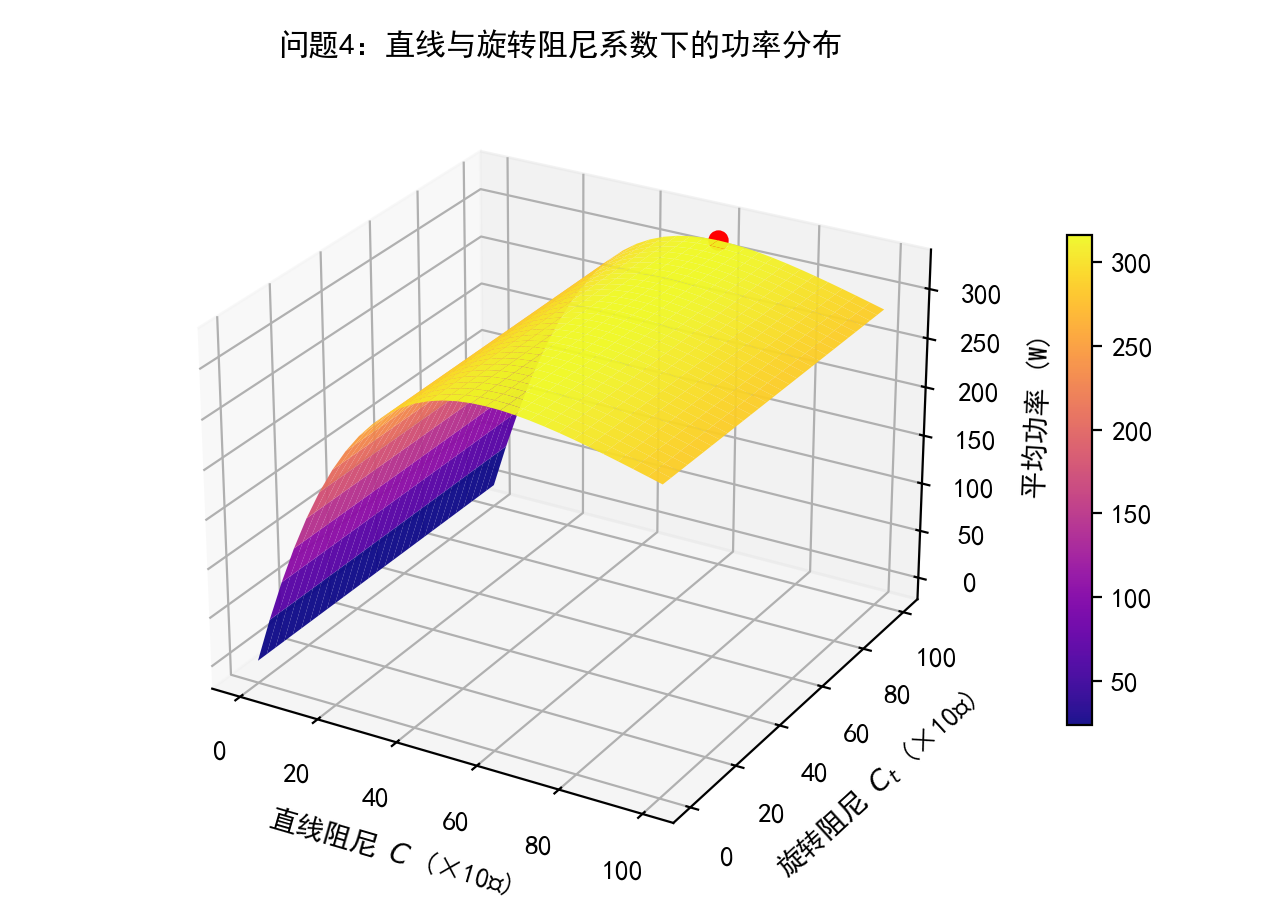
\includegraphics[width=\textwidth]{Figure/fig_sim_08.png}
		\end{center}
		\column{0.5\textwidth}
		\remark{我的想法}{沿旋转阻尼方向几乎一马平川，沿直线阻尼方向才有峰值——参数分``敏感''和``不敏感''，优化要抓大放小。我复现 316.50W，和论文很接近。}
	\end{columns}
\end{frame}

\section{模型检验（分析）思考}
\begin{frame}
	\frametitle{模型检验（一）：检验原理与垂荡检验}
	\scriptsize
	\begin{columns}[T]
		\column{0.5\textwidth}
		\begin{block}{检验原理}
			\begin{itemize}
				\item 装置属\textbf{简谐激励下线性系统的受迫振动}，稳定后振动周期应与波浪激励周期接近
				\item 比较实际响应周期与理论激励周期的方差 $\delta$，$\delta$ 小则模型正确
			\end{itemize}
		\end{block}
		\begin{block}{垂荡模型检验结果}
			\begin{itemize}
				\item 题 1.(1)：$\delta=0.0017<0.1\%$
				\item 题 1.(2)：$\delta=0.0034<0.4\%$
			\end{itemize}
		\end{block}
		\column{0.5\textwidth}
		\begin{center}
			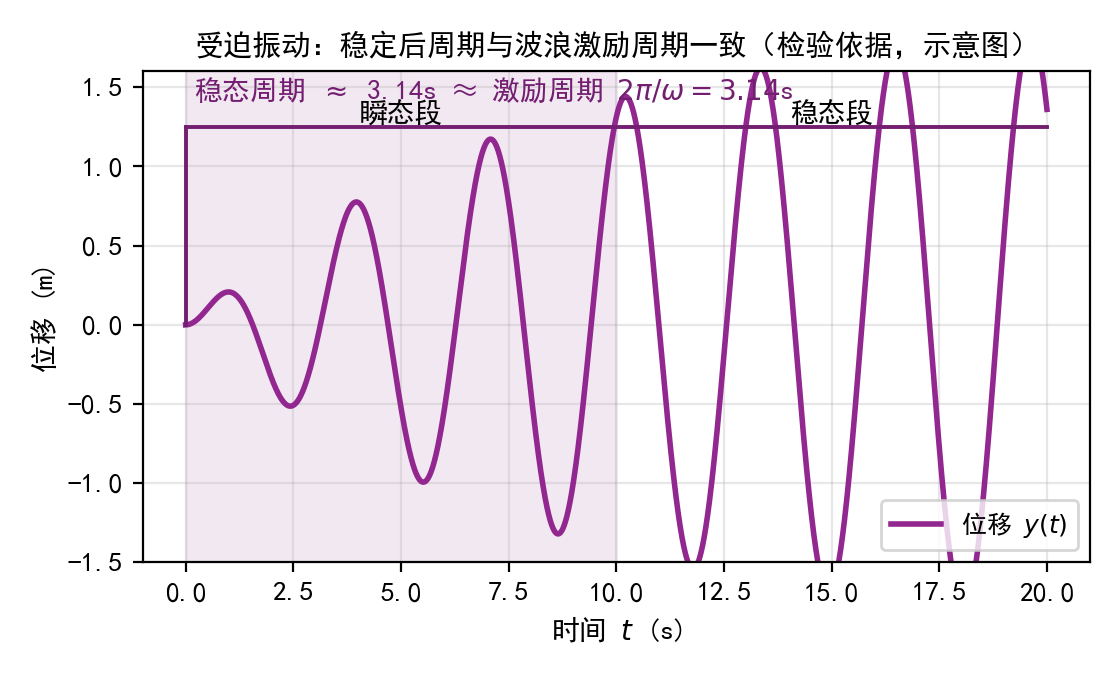
\includegraphics[height=0.45\textheight]{Figure/fig_forced.png}\\
			\scriptsize 受迫振动稳态周期约等于激励周期（示意）
		\end{center}
		\remarkg{我的想法}{以前我总以为检验得靠实验数据，看了这篇才明白：没有实验也能验——用物理常识。受迫振动稳定后周期必等于激励周期，拿它一对就知道模型对不对。}
	\end{columns}
\end{frame}

\begin{frame}
	\frametitle{模型检验（二）：纵摇检验与可靠性检验}
	\scriptsize
	\begin{columns}[T]
		\column{0.5\textwidth}
		\begin{block}{纵摇模型检验结果}
			题 3：$\delta=0.00036<0.04\%$，方差极小，认为模型正确
		\end{block}
		\begin{block}{结果可靠性检验}
			\begin{itemize}
				\item 问题三要算浮子转动惯量，可能引入误差
				\item 对问题三参数加 $\pm 1\%$ 扰动，比较扰动前后输出偏差
				\item 偏差 $<0.10\%$，结果对参数不敏感，求解可靠
			\end{itemize}
		\end{block}
		\column{0.5\textwidth}
		\begin{center}
			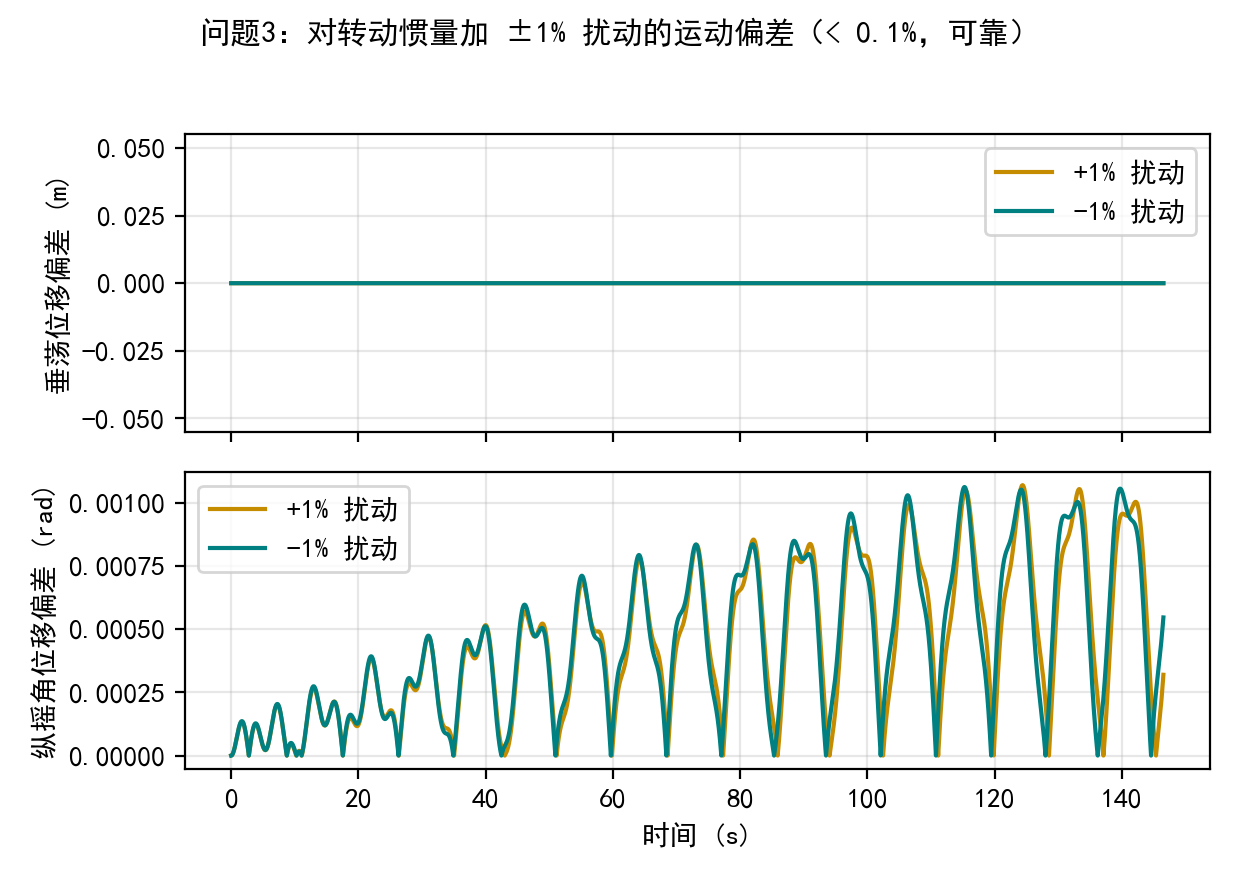
\includegraphics[height=0.44\textheight]{Figure/fig_sim_09.png}\\
			\scriptsize 对转动惯量加 $\pm1\%$ 扰动后的运动偏差
		\end{center}
		\remarkp{我的想法}{我亲手把转动惯量加 $\pm1\%$ 重算，偏差确实很小。模型对参数不敏感，结果才值得相信，这个``扰动检验''以后我也要用。}
	\end{columns}
\end{frame}

\begin{frame}
	\frametitle{模型检验（三）：小结}
	\scriptsize
	\begin{itemize}
		\item 检验的尺子是物理常识（周期该吻合），不是自己说了算
		\item 查了方程对不对（周期方差），也查了结果稳不稳（参数扰动）
		\item 每个数字都给了阈值（0.1\%、0.4\%、0.04\%、0.10\%），站得住脚
	\end{itemize}
	\remark{我的想法}{写检验得和物理常识挂钩、把阈值写具体，不然光一句“误差很小”没人信。}
\end{frame}

\begin{frame}
	\frametitle{教程：检验别说"误差很小"}
	\scriptsize
	\begin{columns}[T]
		\column{0.5\textwidth}
		\begin{exampleblock}{要这样做}
			\begin{itemize}
				\item 检验标准要可验证：这篇用"周期吻合"这个物理常识
				\item 数字给具体阈值：$\delta<0.1\%$，偏差$<0.10\%$
				\item 既验模型对不对（周期方差），又验结果稳不稳（参数扰动）
				\item 告诉你扰动怎么加的（$\pm1\%$）、加了之后怎么对比的
			\end{itemize}
		\end{exampleblock}
		\column{0.5\textwidth}
		\begin{alertblock}{不要这样做}
			\begin{itemize}
				\item "误差在可接受范围内"——没有数，没人知道可不可
				\item 只验一个case就说"模型正确"
				\item 拿自己的结果跟自己比（循环验证）
				\item 检验跟前面的假设/建模完全无关
			\end{itemize}
		\end{alertblock}
	\end{columns}
	\remark{跟你们说}{评委看检验就看两样：你怎么验的、数字是多少。没有数字的检验等于没写。可以用物理常识当尺子，也可以拿文献数据对比，关键是给值。}
\end{frame}

\section{总结}
\begin{frame}
	\frametitle{总结（一）：模型优点}
	\scriptsize
	\begin{enumerate}
		\item 受力分析是建模的地基，算出来的运动还挺贴近实际
		\item 积分没法解析算，用梯形离散化把难度降了下来
		\item 求解用改进龙格库塔、寻优用遗传算法，两头都有保障
	\end{enumerate}
	\remarkg{我的收获}{读完整篇我最想学的，就是它每一环都踩在点上：建模靠受力分析、算积分靠离散化、求解靠龙格库塔加遗传算法。这三样我也都能学，只是未必一次学得会。}
\end{frame}

\begin{frame}
	\frametitle{总结（二）：模型缺点}
	\scriptsize
	\begin{block}{缺点}
		\begin{enumerate}
			\item \textbf{重心计算有简化}：计算浮子重心时忽略浮子厚度等，可能产生偏差
			\item \textbf{忽略耦合效应}：忽略纵摇与垂荡的耦合，对静水恢复力做了简化；实际运动中两自由度会相互影响
		\end{enumerate}
	\end{block}
	\remarkp{我的思考}{说明作者心里清楚自己模型哪里弱。写缺点这事我以前怕减分，现在看反而加分。}
\end{frame}

\begin{frame}
	\frametitle{总结（三）：模型推广与改进}
	\scriptsize
	\begin{block}{推广}
		\begin{itemize}
			\item 方法可用于其他受波浪激励物体的运动分析，可用遗传算法设计最优阻尼系数，对实际生产有借鉴意义
		\end{itemize}
	\end{block}
	\begin{block}{改进方向}
		\begin{itemize}
			\item 实际运动中不同自由度会互相耦合，后续可建立\textbf{纵摇-垂荡耦合运动模型}
		\end{itemize}
	\end{block}
	\remark{我的想法}{总结别光复述做了啥，得给个“以后还能咋办”的方向，才算有内容。}
\end{frame}

\section{心得与收获}
\begin{frame}
	\frametitle{心得与收获：我带走这五点}
	\scriptsize
	\begin{itemize}
		\item \textbf{审题}：按建模需要拆题干——结构、受力、目标各在哪
		\item \textbf{建模}：先受力分析、再列方程，每一项都能对上受力图
		\item \textbf{方法}：牛顿定律 + 龙格库塔 + 遗传算法，一套打到底
		\item \textbf{优化}：先粗扫再精找，避开局部最优；约束给具体范围
		\item \textbf{检验}：物理常识当标尺（周期吻合），参数扰动验可靠性
	\end{itemize}
	\remark{我的收获}{这五点是我读完整篇最想带走的。建模题不怕方法多，怕的是思路乱——六步走稳，比背一堆模型管用。}
\end{frame}


% ---------- 结束页 ----------
\begin{frame}
	\centering
	\Huge{感谢聆听！}\\[1cm]
	\Large{敬请各位老师、同学批评指正}
\end{frame}

\appendix

\begin{frame}
	\centering
	\vspace{1.5cm}
	{\usebeamerfont{title}\color{orchiddark}附录：振动与数值方法基础}\\
	\vspace{0.5cm}
	{\color{orchidpurple}\rule{0.35\textwidth}{1.2pt}}
\end{frame}

\section*{附录 A：振动理论补充}
\begin{frame}
	\frametitle{振动理论 1/7：简谐振动的三个要素}
	\scriptsize
	\begin{block}{简谐振动}
		\begin{center}
			$x(t)=A\cos(\omega t+\varphi)$
		\end{center}
		\begin{itemize}
			\item \textbf{振幅} $A$：振动的最大偏离量
			\item \textbf{圆频率} $\omega$：$\omega=2\pi/T$，一圈对应 $2\pi$
			\item \textbf{周期与频率}：$T=2\pi/\omega$，$f=1/T$（题里说的频率其实指 $\omega$，即圆频率）
		\end{itemize}
	\end{block}
	\begin{block}{和本题的关系}
		波浪激励力 $f\cos\omega t$ 就是一个简谐力，周期固定为 $T=2\pi/\omega$，浮子振子就绕着这个周期来回动
	\end{block}
	\remark{我的想法}{我上学时老把周期和频率搞混，后来记成：周期是``一圈多久''，频率是``一秒几圈''，$\omega$ 就是频率乘 $2\pi$。}
\end{frame}

\begin{frame}
	\frametitle{振动理论 2/7：单自由度自由振动}
	\scriptsize
	\begin{block}{弹簧-质量系统}
		\begin{center}
			$m\ddot x + kx = 0$，自然频率 $\omega_n=\sqrt{\dfrac{k}{m}}$
		\end{center}
		解：$x(t)=A\cos(\omega_n t+\varphi)$，只由系统的质量、刚度决定，与外界无关
	\end{block}
	\begin{block}{两条腿}
		\begin{itemize}
			\item \textbf{质量} $m$：惯性，让物体"懒得起停"
			\item \textbf{刚度} $k$：恢复力，把物体往平衡位置拉
		\end{itemize}
	\end{block}
	\remark{我的想法}{自然频率是个很有意思的量：同样一根弹簧，挂的重物越沉，晃得越慢。这题里浮子的``自然频率''就由质量和静水恢复力决定。}
\end{frame}

\begin{frame}
	\frametitle{振动理论 3/7：阻尼振动三种形态}
	\scriptsize
	\begin{columns}[T]
		\column{0.55\textwidth}
		\begin{block}{阻尼比}
			\begin{center}
				$\zeta=\dfrac{c}{2\sqrt{mk}}$
			\end{center}
			\begin{itemize}
				\item $\zeta<1$：\textbf{欠阻尼}，越振越小，慢慢衰减
				\item $\zeta=1$：\textbf{临界阻尼}，最快回到平衡
				\item $\zeta>1$：\textbf{过阻尼}，慢吞吞地回到平衡
			\end{itemize}
		\end{block}
		\begin{exampleblock}{和本题的关系}
			阻尼系数 $C$ 就是这里的 $c$。后面问题二、四"求最优阻尼"，本质就是在调这个 $\zeta$
		\end{exampleblock}
		\column{0.45\textwidth}
		\begin{center}
		\begin{tikzpicture}[scale=0.82]
			\draw[->] (0,0) -- (7.0,0) node[below,font=\scriptsize] {$t$};
			\draw[->] (0,-1.25) -- (0,1.25) node[left,font=\scriptsize] {$x$};
			\draw[domain=0:6.6,samples=140,smooth,thick,orchidpurple] plot (\x,{exp(-0.2*\x)*cos(2.2*\x r)});
			\draw[domain=0:6.6,samples=60,smooth,thick,teal] plot (\x,{exp(-1.4*\x)});
			\draw[domain=0:6.6,samples=60,smooth,thick,orchidgold] plot (\x,{exp(-2.6*\x)});
			\node[anchor=west,font=\scriptsize,orchidpurple] at (4.4,0.55) {欠阻尼 $\zeta<1$};
			\node[anchor=west,font=\scriptsize,teal] at (4.4,0.10) {临界 $\zeta=1$};
			\node[anchor=west,font=\scriptsize,orchidgold] at (4.4,-0.6) {过阻尼 $\zeta>1$};
		\end{tikzpicture}
		\end{center}
	\end{columns}
\end{frame}

\begin{frame}
	\frametitle{振动理论 4/7：受迫振动}
	\scriptsize
	\begin{block}{方程}
		\begin{center}
			$m\ddot x + c\dot x + kx = F\cos\omega t$
		\end{center}
		解 = \textbf{瞬态解}（初始扰动引起，慢慢衰减消失）+ \textbf{稳态解}（以激励频率 $\omega$ 振荡）
	\end{block}
	\begin{block}{关键结论}
		\begin{itemize}
			\item 稳态后振动的\textbf{频率一定等于激励频率} $\omega$，和系统自然频率无关
			\item 这正是论文\textbf{模型检验}的根据：稳态周期 $=$ 激励周期，对得上就说明模型没建错
		\end{itemize}
	\end{block}
	\remark{我的想法}{我第一次看论文的检验方法时觉得很妙：不用实验数据，靠"受迫振动频率必等于激励频率"这条物理铁律就能验模型。}
\end{frame}

\begin{frame}
	\frametitle{振动理论 5/7：幅频特性与共振}
	\scriptsize
	\begin{block}{稳态振幅}
		\begin{center}
			$A(\omega)=\dfrac{F}{\sqrt{(k-m\omega^2)^2+(c\omega)^2}}$
		\end{center}
		\begin{itemize}
			\item 激励频率 $\omega$ 接近自然频率 $\omega_n$ 时，振幅被放大
			\item 阻尼越小，放大越狠，共振峰越高
		\end{itemize}
	\end{block}
	\begin{block}{和本题的关系}
		波浪装置要让浮子振幅大、又别失控，频率设计就要避开共振区；阻尼也不能太小，否则峰太高把装置晃散架
	\end{block}
	\remark{我的想法}{共振这事我理解成：推秋千要在对的时间点用力，频率对上了，几下就荡很高。}
\end{frame}

\begin{frame}
	\frametitle{振动理论 6/7：三个水动力项在方程里的角色}
	\scriptsize
	\begin{block}{附加惯性力（附加质量 $m_a$）}
		浮子一动要推开周围的海水，等于额外背了一团水，方程里体现为 $(m_1+m_a)\ddot x$
	\end{block}
	\begin{block}{兴波阻尼力（系数 $B_v$）}
		浮子晃动会兴起波浪，能量随波跑掉，起的是"阻尼"作用，方程里是 $-B_v\dot x$
	\end{block}
	\begin{block}{静水恢复力（$-\rho g A x$）}
		浮子偏离平衡，吃水变化带来浮力差，把它往回拉，作用像弹簧，方程里是 $-\rho g A x$
	\end{block}
	\remark{我的想法}{这三个力其实是"惯性的额外负担、能量的损耗、位置的拉回"，对应方程的三类项，记起来就不乱了。}
\end{frame}

\begin{frame}
	\frametitle{振动理论 7/7：微幅波与线性化}
	\scriptsize
	\begin{block}{线性周期微幅波}
		\begin{itemize}
			\item \textbf{微幅}：波高远小于波长，水面斜率很小
			\item 于是作用在浮子上的力近似\textbf{与位移、速度成正比}，方程是线性的
		\end{itemize}
	\end{block}
	\begin{block}{线性化的好处}
		\begin{itemize}
			\item 线性方程可\textbf{叠加}：几个波的作用可以分开算再相加
			\item 受力分析能一项一项写清楚（激励、附加、兴波、静水恢复）
			\item 后面才能用矩阵、状态空间那套工具
		\end{itemize}
	\end{block}
	\remark{我的想法}{假设里那句``海水无粘、无旋''其实是为这条服务的：无粘无旋才能用势流理论把波浪力解析地求出来。}
\end{frame}

\section*{附录 B：数值方法补充}
\begin{frame}
	\frametitle{数值方法 1/8：为什么要数值求解}
	\scriptsize
	\begin{block}{微分方程不是都能解析解}
		\begin{itemize}
			\item 多数实际方程没有闭式解；就算有，想求某一时刻的具体数值也麻烦
			\item 数值方法换了个思路：\textbf{从初值出发，一步一个小步长往前推}
		\end{itemize}
	\end{block}
	\begin{block}{核心思想}
		\begin{center}
			$y_{n+1}=y_n+\text{(步长)}\times\text{(斜率估计)}$
		\end{center}
		后面欧拉、龙格库塔，全是在"怎么把这个斜率估准"上做文章
	\end{block}
	\remark{我的想法}{我第一次学数值解时总觉得是"笨办法"，后来才懂：解析解求不出的时候，数值解就是唯一的路，而且还能控制精度。}
\end{frame}

\begin{frame}
	\frametitle{数值方法 2/8：欧拉法}
	\scriptsize
	\begin{block}{公式}
		\begin{center}
			$y_{n+1}=y_n+h\,f(t_n,y_n)$
		\end{center}
		几何：用\textbf{起点的切线}代替曲线走一步
	\end{block}
	\begin{block}{精度}
		\begin{itemize}
			\item 每步误差约 $O(h^2)$，整体 $O(h)$，叫\textbf{一阶精度}
			\item 步长 $h$ 大一点，误差就明显；步长小，步数暴涨
		\end{itemize}
	\end{block}
	\begin{block}{为什么不用它}
		40 个周期、要 0.2s 间隔的精确结果，欧拉法要么精度不够、要么算到天荒地老，所以论文用更高阶的方法
	\end{block}
	\remark{我的想法}{欧拉法简单，但我印象里它特别"脆"：参数稍微差一点结果就飘，老师讲数值分析时反复拿它开刀。}
\end{frame}

\begin{frame}
	\frametitle{数值方法 3/8：改进欧拉（中点法）}
	\scriptsize
	\begin{block}{预测-校正}
		\begin{enumerate}
			\item 先用欧拉法\textbf{预测}中点的值：$y_{n+1/2}\approx y_n+\frac{h}{2}f(t_n,y_n)$
			\item 再用\textbf{中点斜率}校正走完整步长：$y_{n+1}=y_n+h\,f(t_{n+1/2},y_{n+1/2})$
		\end{enumerate}
	\end{block}
	\begin{block}{精度}
		用中点斜率代替起点斜率，每步误差降到 $O(h^3)$，整体 $O(h^2)$，\textbf{二阶精度}
	\end{block}
	\remark{我的想法}{"先猜一步、再回头校准"，这个思路叫预测-校正，龙格库塔就是把它做到极致。}
\end{frame}

\begin{frame}
	\frametitle{数值方法 4/8：龙格库塔的思想}
	\scriptsize
	\begin{columns}[T]
		\column{0.5\textwidth}
		\begin{block}{多取几个斜率加权}
			\begin{itemize}
				\item $k_1$：起点斜率
				\item $k_2$：用 $k_1$ 预测到中点，取中点斜率
				\item $k_3$：用 $k_2$ 再修一次中点斜率
				\item $k_4$：用 $k_3$ 预测到终点，取终点斜率
			\end{itemize}
		\end{block}
		\column{0.5\textwidth}
		\begin{center}
			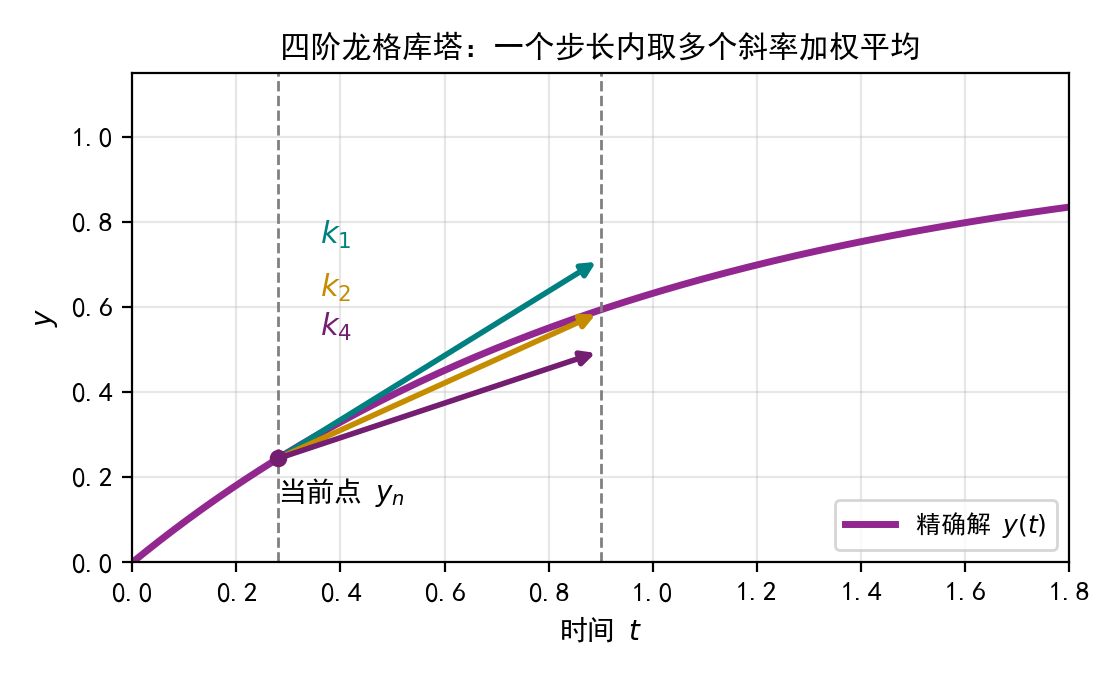
\includegraphics[height=0.26\textheight]{Figure/fig_rk4.png}
		\end{center}
		\begin{block}{直觉}
			一步里多问几个点"斜率是多少"，再按权重平均，曲线就跟得更准
		\end{block}
	\end{columns}
\end{frame}

\begin{frame}
	\frametitle{数值方法 5/8：四阶龙格库塔公式与精度}
	\scriptsize
	\begin{block}{递推公式}
		\begin{center}
			$y_{n+1}=y_n+\dfrac{h}{6}(k_1+2k_2+2k_3+k_4)$
		\end{center}
		$k_1=f(t_n,y_n)$，\ $k_2=f(t_n+\frac{h}{2},y_n+\frac{h}{2}k_1)$，\ $k_3=f(t_n+\frac{h}{2},y_n+\frac{h}{2}k_2)$，\ $k_4=f(t_n+h,y_n+h k_3)$
	\end{block}
	\begin{block}{精度}
		\begin{itemize}
			\item 每步误差 $O(h^5)$，整体 $O(h^4)$，叫\textbf{四阶}
			\item 步长减半，误差大约缩到原来的 $1/16$
		\end{itemize}
	\end{block}
	\remark{我的想法}{论文把步长取到 $10^{-4}$，就是在精度和速度之间折中的结果：再大 40 个周期就抖，再小就算不动。}
\end{frame}

\begin{frame}
	\frametitle{数值方法 6/8：高阶方程转一阶方程组}
	\scriptsize
	\begin{block}{状态变量法}
		二阶方程 $m\ddot x+c\dot x+kx=F(t)$，令状态 $\bm y=\begin{pmatrix}x\\ \dot x\end{pmatrix}$，改写为
		\begin{center}
			$\dfrac{d}{dt}\bm y=\begin{pmatrix}\dot x\\ \frac{1}{m}(F(t)-c\dot x-kx)\end{pmatrix}$
		\end{center}
		变成两个一阶方程，龙格库塔直接套用
	\end{block}
	\begin{block}{本题的规模}
		\begin{itemize}
			\item 问题一（垂荡）：浮子+振子，共 \textbf{4 个一阶方程}
			\item 问题三（垂荡+纵摇）：4 个量变 8 个，\textbf{8 个一阶方程}
		\end{itemize}
	\end{block}
	\remark{我的想法}{别被"8 个方程"吓到，本质和 1 个没区别，就是数组变长了，递推公式一个字都不用改。}
\end{frame}

\begin{frame}
	\frametitle{数值方法 7/8：数值积分——梯形法}
	\scriptsize
	\begin{columns}[T]
		\column{0.5\textwidth}
		\begin{block}{把积分变成求和}
			\begin{itemize}
				\item 平均功率是积分，但 $P(t)$ 只有离散的数值解
				\item 梯形法：用一个个\textbf{小梯形}的面积近似曲线下的面积
				\item 步长越小，梯形越贴近曲线，结果越准
			\end{itemize}
		\end{block}
		\column{0.5\textwidth}
		\begin{center}
			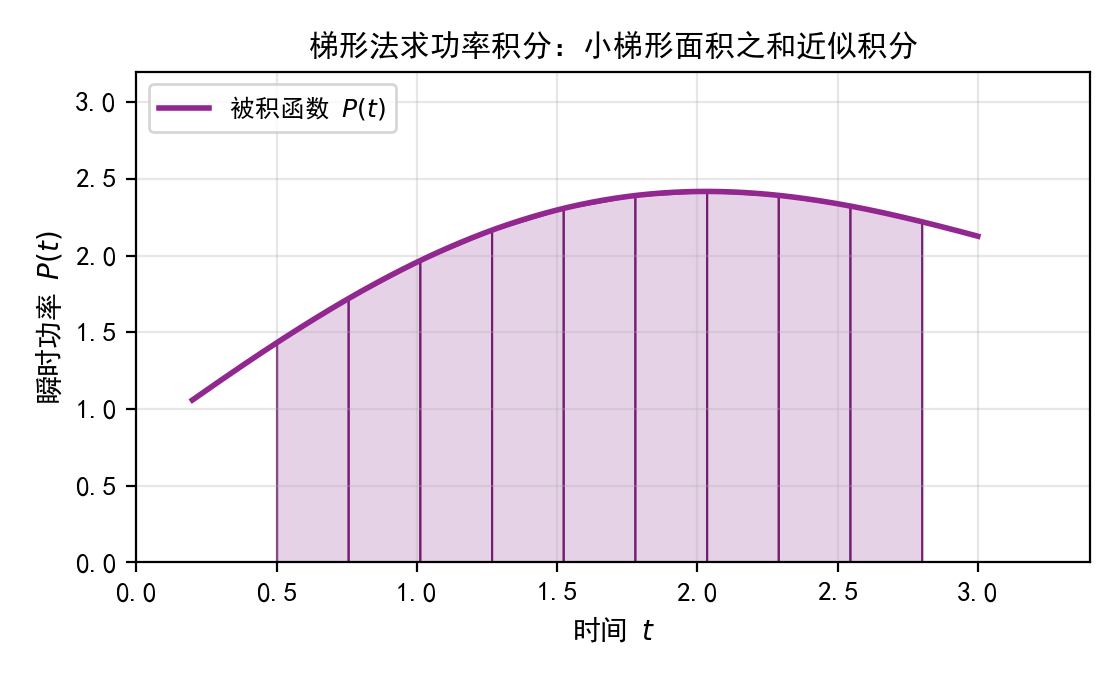
\includegraphics[height=0.26\textheight]{Figure/fig_sim_04.png}
		\end{center}
		\begin{block}{应用}
			论文算平均功率就是取稳态段 $[100,180]$s，用梯形法把 $P(t)$ 离散求和
		\end{block}
	\end{columns}
\end{frame}

\begin{frame}
	\frametitle{数值方法 8/8：遗传算法}
	\scriptsize
	\begin{block}{模拟自然选择}
		\begin{itemize}
			\item \textbf{种群}：一批候选解（一组阻尼系数）
			\item \textbf{适应度}：就是平均输出功率，功率大的"活得好"
			\item \textbf{选择/交叉/变异}：好的解留下、互相"杂交"、偶尔"变异"出新解
		\end{itemize}
	\end{block}
	\begin{block}{为什么用它优化}
		\begin{itemize}
			\item 暴力遍历 $[0,100000]$ 太慢，还要撞运气
			\item 遗传算法\textbf{并行搜索、概率选择}，不容易卡在局部最优
			\item 论文用它配合"先粗扫"，又快又不漏
		\end{itemize}
	\end{block}
	\remark{我的想法}{我第一次看遗传算法觉得像玄学，后来明白它就是把"优胜劣汰"搬进计算机，多迭代几代自然逼近最优。}
\end{frame}

\begin{frame}
	\frametitle{遗传算法专题 1/4：算法流程}
	\scriptsize
	\begin{columns}[c]
		\column{0.45\textwidth}
		\begin{center}
		\begin{tikzpicture}[
			gabox/.style={draw=orchidpurple, thick, rounded corners=3pt,
				minimum width=2.7cm, minimum height=0.85cm, align=center,
				fill=orchidlight!35, font=\scriptsize},
			garr/.style={-stealth, thick, orchidpurple},
			scale=0.82
		]
			\node[gabox] (a) at (0,0) {初始化种群};
			\node[gabox] (b) at (0,-1.5) {适应度评估\\（平均输出功率）};
			\node[gabox] (c) at (0,-3.0) {选择、交叉、变异};
			\node[gabox] (d) at (0,-4.5) {满足终止条件？};
			\node[gabox, fill=orchidpurple, text=white] (e) at (3.7,-4.5) {输出最优阻尼};
			\draw[garr] (a.south) -- (b.north);
			\draw[garr] (b.south) -- (c.north);
			\draw[garr] (c.south) -- (d.north);
			\draw[garr] (d.east) -- (e.west) node[midway, above, font=\scriptsize]{是};
			\draw[garr] (d.west) -- ++(-1.3,0) -- ++(0,3.0) -- (b.west) node[midway, left, font=\scriptsize]{否};
		\end{tikzpicture}
		\end{center}
		\column{0.55\textwidth}
		\begin{block}{关键在哪}
			\begin{itemize}
				\item 一开始是\textbf{随机}的一批解，谁好谁坏不知道
				\item 每一代都按适应度``淘汰差的、留下好的''
				\item 反复迭代几百代，种群整体向功率高的区域靠拢
			\end{itemize}
		\end{block}
		\remark{我的想法}{遗传算法的套路很像人：先瞎试，再择优、杂交、偶尔突变，一代代下来越来越好。}
	\end{columns}
\end{frame}

\begin{frame}
	\frametitle{遗传算法专题 2/4：三个基本算子}
	\scriptsize
	\begin{block}{选择（轮盘赌）}
		适应度（功率）越高的个体，被选中``传宗接代''的概率越大——就像转盘，面积越大越容易停到
	\end{block}
	\begin{block}{交叉（单点）}
		把两条解在某个位置``切开''再交换后半段，产生两条新解，相当于父代的基因重组
	\end{block}
	\begin{block}{变异（随机扰动）}
		小概率把某个基因值随机改一下，防止种群太像、原地踏步
	\end{block}
	\remark{我的想法}{三个算子各有分工：选择保证"越好的越容易留下来"，交叉制造新组合，变异负责"偶尔跳出去"防止卡死。}
\end{frame}

\begin{frame}
	\frametitle{遗传算法专题 3/4：为什么不容易卡在局部最优}
	\scriptsize
	\begin{block}{三个原因}
		\begin{itemize}
			\item \textbf{并行}：种群同时盯着很多个点，不像贪心只盯着一个方向爬
			\item \textbf{概率}：差的个体只是"概率低"，不是彻底没机会，多样性保住了
			\item \textbf{变异}：随机扰动让种群有机会从``坑''里跳出去
		\end{itemize}
	\end{block}
	\begin{block}{对比暴力遍历}
		暴力遍历把 $[0,100000]$ 一个点一个点算，又慢又没方向；遗传算法直接"奔着高的地方去"，快好几个数量级
	\end{block}
	\remark{我的想法}{以前我觉得"搜索"就是把所有可能试一遍，遗传算法让我开了眼：原来可以带着一群候选解"有方向地"找。}
\end{frame}

\begin{frame}
	\frametitle{遗传算法专题 4/4：在本题里的用法}
	\scriptsize
	\begin{columns}[c]
		\column{0.5\textwidth}
		\begin{center}
			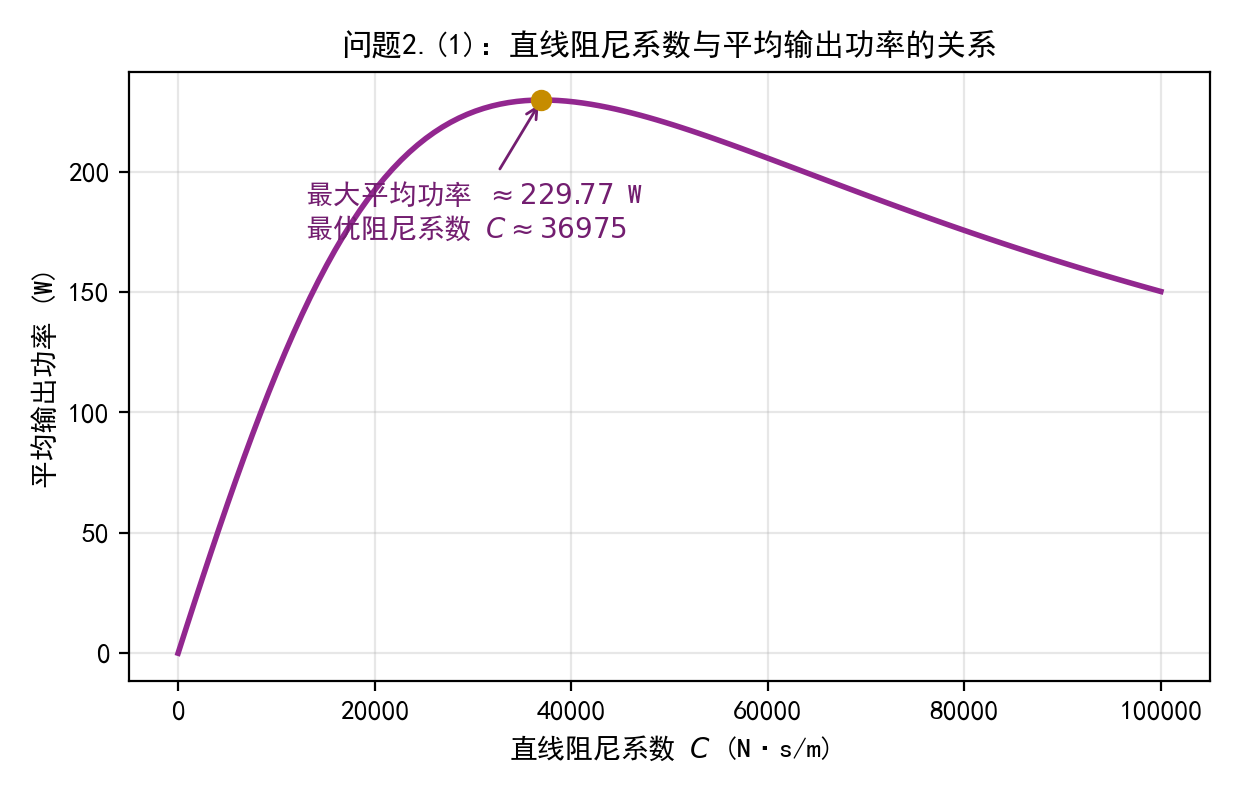
\includegraphics[width=\textwidth]{Figure/fig_sim_05.png}
		\end{center}
		\column{0.5\textwidth}
		\begin{block}{映射关系}
			\begin{itemize}
				\item \textbf{个体（基因）}：阻尼系数 $C$（或 $(\alpha,\beta)$、$(C,C_t)$）
				\item \textbf{适应度}：该阻尼下的平均输出功率
				\item \textbf{约束}：$C\in[0,100000]$ 等，就编码在种群范围里
			\end{itemize}
		\end{block}
		\begin{block}{论文的做法}
			先粗扫找到大致范围，再用遗传算法\textbf{迭代 200 代}精确锁定峰顶，得到 $C\approx37186$、$P\approx229.77$W
		\end{block}
		\remark{我的想法}{图里的单峰就是遗传算法的``地形''，种群一代代往峰顶爬，最后停在最高处。}
	\end{columns}
\end{frame}

\end{document}
